\documentclass[a4paper]{article}
\usepackage[UTF8]{ctex}
\usepackage[a4paper,margin=1in]{geometry}
\usepackage{graphicx}
\usepackage{float}
\usepackage{listings}
\usepackage{booktabs}
\usepackage{hyperref}
\usepackage{fancyhdr}
\usepackage{lastpage}
\usepackage{color}
\usepackage{xcolor}
\usepackage{indentfirst}
\setlength{\parindent}{2em}
\usepackage{zhnumber}
\usepackage[dvipsnames]{xcolor}
\usepackage{amsmath}
\usepackage{multirow}
\usepackage{tikz}
\usetikzlibrary{shapes,arrows,positioning}

% ===== 个人信息与实验信息配置 =====
\newcommand{\projname}{ROSE——编译原理逆向工程工具}
\newcommand{\reporttitle}{实验二-设计文档}
\newcommand{\stuno}{23336179}
\newcommand{\authorname}{马福泉}
\newcommand{\major}{计算机科学与技术}
\newcommand{\adviser}{李文军}
\newcommand{\startdate}{2026年6月}
\newcommand{\labenddate}{2026年6月}
\newcommand{\labroom}{B203}

% ===== 页眉页脚设置 =====
\pagestyle{fancy}
\fancyhf{}
\fancyhead[L]{\kaishu \projname}
\fancyhead[C]{\kaishu \reporttitle}
\fancyhead[R]{\kaishu \authorname}
\fancyfoot[C]{第 \thepage 页，共 \pageref{LastPage} 页}
\renewcommand{\headrulewidth}{0.4pt}
\renewcommand{\footrulewidth}{0pt}

% ===== 代码高亮配置 =====
\definecolor{NavyBlue}{RGB}{0,0,128}
\definecolor{codegreen}{RGB}{0,128,0}
\definecolor{codegray}{RGB}{128,128,128}
\definecolor{codepurple}{RGB}{128,0,128}
\definecolor{backcolour}{RGB}{245,245,245}

\lstset{
    language=Java,
    basicstyle=\ttfamily\small,
    commentstyle=\color{codegreen}\itshape,
    keywordstyle=\color{NavyBlue}\bfseries,
    stringstyle=\color{codepurple},
    numberstyle=\tiny\color{codegray},
    backgroundcolor=\color{backcolour},
    breaklines=true,
    frame=single,
    numbers=left,
    tabsize=4,
    showstringspaces=false,
    captionpos=b,
    escapeinside={\%}{\%},
    morekeywords={enum,record}
}

\begin{document}

% ==================== 封面 ====================
\begin{titlepage}
    \centering
    
    
\includegraphics[width=10cm]{img/SYSULogo.png}

    \vspace{1em}
    {\Large \kaishu \projname \par}
    \vspace{3em}

    {\fontsize{36pt}{40pt}\kaishu \selectfont \boldmath \reporttitle\par}
    \vspace{2em}
    \vspace*{\fill}

    \begin{center}
    {\Large
    \makebox[5em][s]{学号}:\underline{\makebox[15em][c]{\kaishu \stuno}}\\[1em]
    \makebox[5em][s]{姓名}:\underline{\makebox[15em][c]{\kaishu \authorname}}\\[1em]
    \makebox[5em][s]{专业}:\underline{\makebox[15em][c]{\kaishu \major}}\\[1em]
    \makebox[5em][s]{指导教师}:\underline{\makebox[15em][c]{\kaishu \adviser}}\\[1em]
    \makebox[5em][s]{起始日期}:\underline{\makebox[15em][c]{\kaishu \startdate}}\\[1em]
    \makebox[5em][s]{结束日期}:\underline{\makebox[15em][c]{\kaishu \labenddate}}\\[1em]
    \makebox[5em][s]{实验地点}:\underline{\makebox[15em][c]{\kaishu \labroom}}
    }
    \end{center}

    \vspace*{\fill}
\end{titlepage}

% ==================== 目录 ====================
\tableofcontents
\newpage

% ==================== 正文 ====================

\section{实验简述}

本项目 ROSE 是一个编译原理逆向工程工具，旨在对 Oberon-0 语言源程序进行词法分析、语法分析、
语义分析，并自动生成流程图和调用关系图。本实验为第二阶段——使用 JFlex 工具自动生成词法
分析器 OberonScanner，实现对 Oberon-0 源程序的词法单元识别与错误检测。

\section{Oberon-0 词汇表}

Oberon-0 的词汇体系可划分为保留字、预定义关键字、运算符与分界符、标识符、字面量及注释
六大类别。表~\ref{tab:vocab} 列出了完整的词汇表。

\begin{table}[H]
\centering
\caption{Oberon-0 完整词汇表}
\label{tab:vocab}
\begin{tabular}{@{}ll@{}}
\toprule
\textbf{类别} & \textbf{词汇} \\
\midrule
\multirow{3}{*}{保留字}
& MODULE, BEGIN, END, IF, THEN, ELSIF, ELSE, WHILE, DO \\
& PROCEDURE, VAR, CONST, TYPE, RECORD, ARRAY, OF \\
& DIV, MOD, OR, \~{} \\
\midrule
预定义关键字 & INTEGER, BOOLEAN, TRUE, FALSE, Read, Write, WriteLn \\
\midrule
\multirow{5}{*}{运算符与分界符}
& +, -, *, DIV, MOD \quad（算术）\\
& =, \#, <, <=, >, >= \quad（关系）\\
& \&, OR, \~{} \quad（逻辑）\\
& :=, :, ;, .\ , , \quad（赋值与分界）\\
& (, ), [, ] \quad（括号）\\
\midrule
标识符 & \{Letter\}(\{Letter\}$\mid$\{Digit\})*, 长度 $\leq$ 24 \\
\midrule
\multirow{2}{*}{字面量}
& 十进制整数: 0 $\mid$ [1-9]\{Digit\}* \\
& 八进制整数: 0[0-7]+ \\
\midrule
注释 & (* ... *) \quad（不可嵌套）\\
\bottomrule
\end{tabular}
\end{table}

\section{正则定义式}

以下以纯文本正则定义式描述 Oberon-0 的词法规则（使用 $\to$ 表示产生、$\epsilon$ 表示空串）：

\begin{itemize}
    \item \textbf{基本符号}
    \begin{verbatim}
    digit  -> 0 | 1 | 2 | 3 | 4 | 5 | 6 | 7 | 8 | 9
    letter -> a | b | ... | z | A | B | ... | Z
    \end{verbatim}

    \item \textbf{空白字符}
    \begin{verbatim}
    whitespace -> ' ' | '\t' | '\r' | '\n'
    \end{verbatim}

    \item \textbf{标识符}
    \begin{verbatim}
    identifier -> letter (letter | digit)*
    \end{verbatim}
    限制：生成的标识符长度必须 $\leq$ 24。

    \item \textbf{整数}
    \begin{verbatim}
    decInteger -> 0 | [1-9] digit*
    octInteger -> 0 (0 | 1 | ... | 7)+
    \end{verbatim}
    约束：(1) 十进制整数首位非零（除非值为 0）；(2) 八进制整数首位必须为 0，且每位 $\in$ [0-7]。

    \item \textbf{注释}
    \begin{verbatim}
    comment     -> "(*" (^("*)"))* "*)"
    \end{verbatim}
    其中 $\texttt{\^{}("*)")}$ 表示除"*\texttt{)}"外的任意字符序列（不支持嵌套）。

    \item \textbf{保留字集合 (Keyword Set K)}
    \begin{verbatim}
    K -> { MODULE, BEGIN, END, IF, THEN, ELSIF, ELSE,
           WHILE, DO, PROCEDURE, VAR, CONST, TYPE,
           RECORD, ARRAY, OF, DIV, MOD, OR, ~ }
    \end{verbatim}
\end{itemize}

\section{词法规则与 C/C++/Java 的异同比较}

Oberon-0 的词法规范与 C/C++/Java 在多个维度上存在显著差异，表~\ref{tab:lex-compare} 给出系统对比。

\begin{table}[H]
\centering
\caption{Oberon-0 与 C/C++/Java 词法差异对比}
\label{tab:lex-compare}
\begin{tabular}{@{}p{4cm}p{5.2cm}p{5.2cm}@{}}
\toprule
\textbf{维度} & \textbf{Oberon-0} & \textbf{C/C++/Java} \\
\midrule
大小写敏感性 & 大小写无关 (case-insensitive)；
所有保留字、标识符忽略大小写 &
大小写敏感；
\texttt{int} 与 \texttt{Int} 是不同的标识符 \\
\midrule
标识符长度限制 & 硬限制 24 字符；超出触发异常 &
C99 $\leq$ 31（内部），Java 无硬性上限 \\
\midrule
注释语法 & 仅支持 \texttt{(* ... *)}，不可嵌套 &
\texttt{//} 单行注释、\texttt{/* ... */} 多行注释 \\
\midrule
整数字面量 & 十进制 + 八进制 (\texttt{0} 前缀)；
八进制含 8/9 触发异常 &
C/Java 支持十进制/八进制(\texttt{0})/十六进制(\texttt{0x}) \\
\midrule
数字-标识符边界 & 强制要求空格分隔；\texttt{123abc} 触发异常 &
C/Java 词法规则中数字后接字母自动作为两个 token \\
\midrule
运算符符号 & \texttt{DIV, MOD, \&, OR, \~, :=, \#} &
\texttt{/, \%, \&\&, ||, !, =, !=} \\
\bottomrule
\end{tabular}
\end{table}

Oberon-0 的关键设计差异可归纳为：

\begin{enumerate}
    \item \textbf{大小写无关}：这是 Pascal 系语言的共同特征，简化了 DFA 状态数量（无需为
    \texttt{A-Z} 和 \texttt{a-z} 分别维护匹配分支）。JFlex 通过 \texttt{\%ignorecase}
    指令一行配置即可生效。

    \item \textbf{标识符长度硬约束}：Oberon-0 的 24 字符上限并非 JFlex 声明式规则所能
    表达，必须在词法动作中以 Java 代码手动检查长度并在超出时抛出
    \texttt{IllegalIdentifierLengthException}。

    \item \textbf{数字-标识符边界强制分离}：C 语言将 \texttt{123abc} 自动拆分为两个
    token（\texttt{123} 和 \texttt{abc}），而 Oberon-0 将其视为词法错误。这是通过
    正则 \texttt{\{Digit\}+\{Letter\}+} 并关联异常抛出实现的——本质上是一种"先匹配
    后拒绝"的策略。

    \item \textbf{八进制整数的严格检查}：Oberon-0 仅接受 \texttt{0[0-7]+}作为有效
    八进制，\texttt{08} 或 \texttt{019} 需被独立的正则模式
    \texttt{0[0-9]*[89]+[0-9]*} 捕获并抛出 \texttt{IllegalOctalException}。

    \item \textbf{注释不支持嵌套}：简化了词法分析器的状态转移逻辑——一个 \texttt{COMMENT}
    状态即可处理，无需维护嵌套深度计数器。
\end{enumerate}

\section{JFlex、JLex、GNU Flex 工具对比}

表~\ref{tab:tool-compare} 从生成语言、算法、性能和功能四个维度对比三种主流词法分析器生成工具。

\begin{table}[H]
\centering
\caption{JFlex vs JLex vs GNU Flex 对比}
\label{tab:tool-compare}
\begin{tabular}{@{}p{3cm}p{3.5cm}p{3.5cm}p{4cm}@{}}
\toprule
\textbf{维度} & \textbf{GNU Flex} & \textbf{JLex} & \textbf{JFlex} \\
\midrule
目标语言 & C / C++ & Java & Java \\
\midrule
首次发布 & 1987 (继承自 Lex) & 1996 & 1998 \\
\midrule
DFA 生成算法 & 表驱动 DFA & 表驱动 DFA & NFA $\to$ DFA 优化；
行压缩表（row-displaced table） \\
\midrule
Unicode 支持 & 有限（依赖 C locale）& 有限（Java 1.0 时代）& \textbf{完整 Unicode 支持}
(基于 Java \texttt{char} 的 16-bit 码点以及代理对) \\
\midrule
正则语法 & POSIX 扩展正则 & 基础正则 & 扩展正则 + 宏定义 +
\textbf{先行断言} + \texttt{\%state} 状态栈 \\
\midrule
性能 & 极高 (C 原生) & 中等 & 高（相比 JLex
提升 2--3 倍扫描速度） \\
\midrule
与 CUP 集成 & 不适用 & 支持 & \textbf{原生支持 CUP}
(\texttt{\%cup} 模式自动生成
\texttt{Symbol} Token) \\
\midrule
维护状态 & 活跃 (GNU 项目) & 停止维护 (1998) & \textbf{活跃维护}
(最新版 1.9+, 2023) \\
\bottomrule
\end{tabular}
\end{table}

\textbf{GNU Flex} 是 Lex 的 GNU 替代品，主导了 C/C++ 生态的词法分析器生成长达三十余年。
其生成的扫描器以 C 语言原生性能著称，但在 Unicode 处理和大字符集场景中表现受限，且不适合
Java 工程集成。

\textbf{JLex} 是普林斯顿大学 Elliot Berk 于 1996 年发布的 Java 版 Lex 移植，首次将
Lex 理念引入 JVM 生态。然而其 DFA 生成算法沿用经典的子集构造法，未做进一步优化；Unicode
支持仅限于 Java 1.0 时期的 \texttt{char} 范围；项目自 1998 年起已停止维护。

\textbf{JFlex} 由 Gerwin Klein 基于 JLex 完全重写，现已成为 Java 生态词法分析器生成的
事实标准。其核心优势包括：(1) 更优的 DFA 压缩算法（行列位移表），生成的分析器性能比 JLex
快 2--3 倍；(2) 完整的 Unicode 支持，允许在正则中直接使用 \texttt{\textbackslash uXXXX}
和 Unicode 类别表达式；(3) 丰富的声明式指令——\texttt{\%ignorecase}、
\texttt{\%state}（独占式/包容式状态）、宏系统——使得词法规则的定义高度模块化；
(4) 与 CUP（Java 版 Yacc）的深度集成，\texttt{\%cup} 模式可直接生成与语法分析器对接的
\texttt{Symbol} Token 流，无需手动编写胶水代码。

本实验选择 JFlex 作为词法分析器生成工具，既因其作为 Java 生态最成熟的 Lex 变体，能无缝
融入 ROSE 工具链的 Java 技术栈；也因其丰富的状态管理能力和异常检测机制（通过词法动作中
的 Java 代码注入）恰好满足 Oberon-0 对标识符长度、数字-标识符边界、八进制合法性等细粒度
错误检测的特殊需求。

\section{JFlex 生成与编译结果}

\begin{figure}[H]
\centering
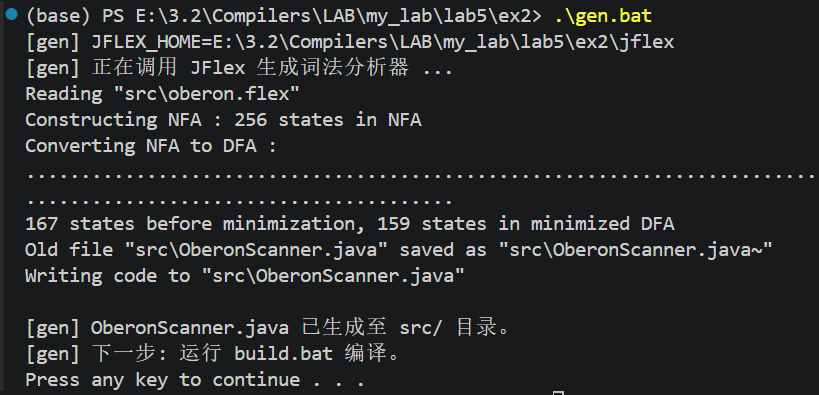
\includegraphics[width=0.9\textwidth]{img/gen_ok.png}
\caption{gen.bat 执行结果：256 NFA 状态 → 159 最小化 DFA 状态}
\label{fig:gen-ok}
\end{figure}

\begin{figure}[H]
\centering
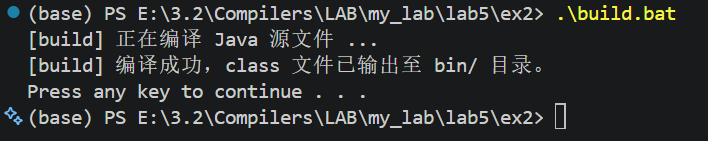
\includegraphics[width=0.9\textwidth]{img/build_ok.png}
\caption{build.bat 执行结果：Token.java + exceptions + OberonScanner.java 全部编译通过}
\label{fig:build-ok}
\end{figure}

\section{变异测试验证}

使用实验一中构造的 8 个变异文件对 OberonScanner 进行错误检测能力验证。图~\ref{fig:mut1}
至图~\ref{fig:mut8} 展示了各变异文件的扫描结果——词法级别的 4 种错误全部被正确捕获并
抛出对应异常，语法和语义级别的错误在词法阶段正常通过（留待后续实验处理）。

\begin{figure}[H]
\centering
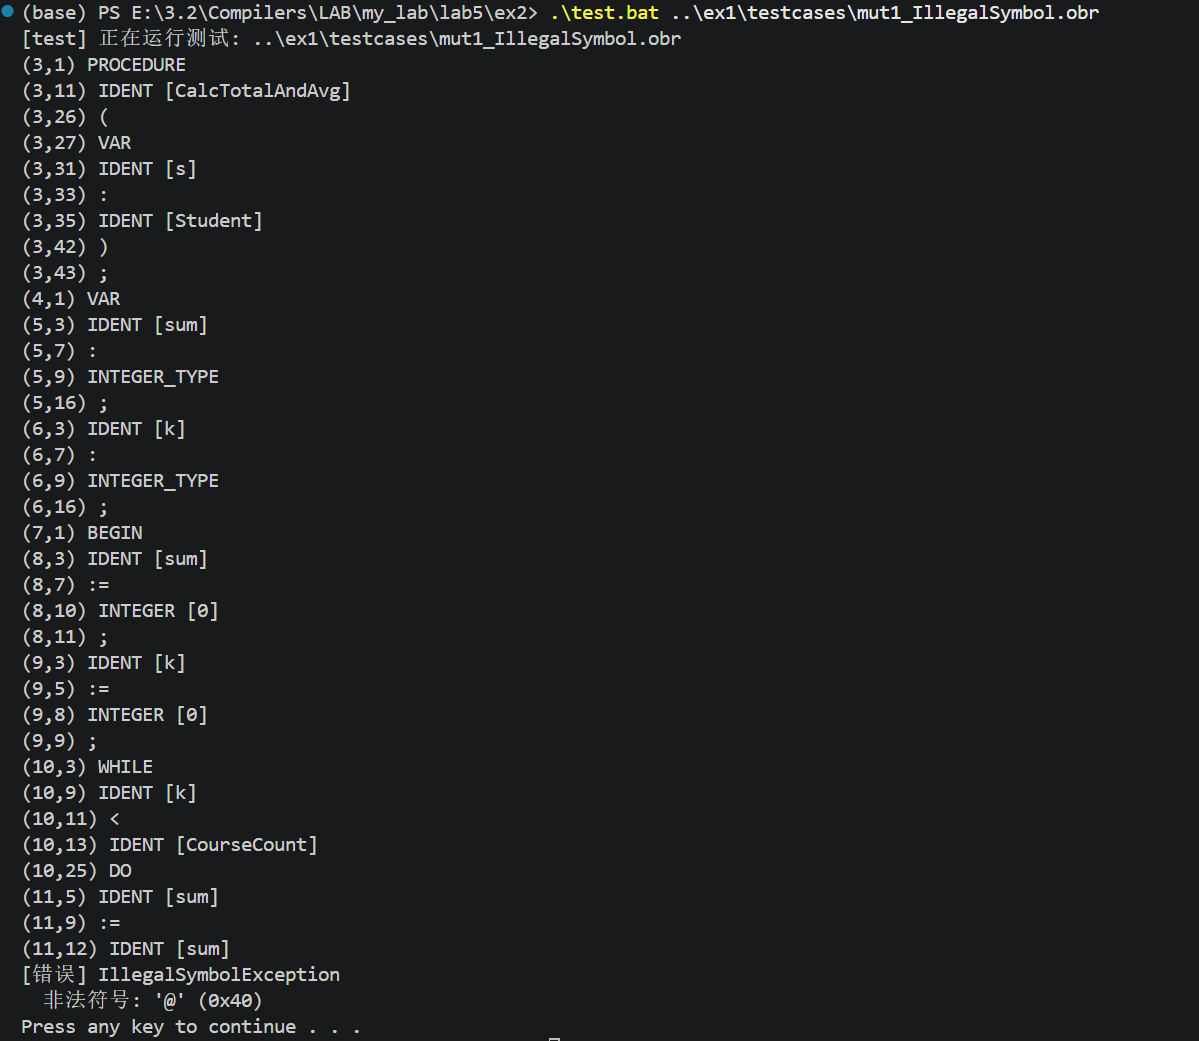
\includegraphics[width=0.9\textwidth]{img/1.png}
\caption{变异 1: IllegalSymbol —— 非法符号 @ 被正确捕获}
\label{fig:mut1}
\end{figure}

\begin{figure}[H]
\centering
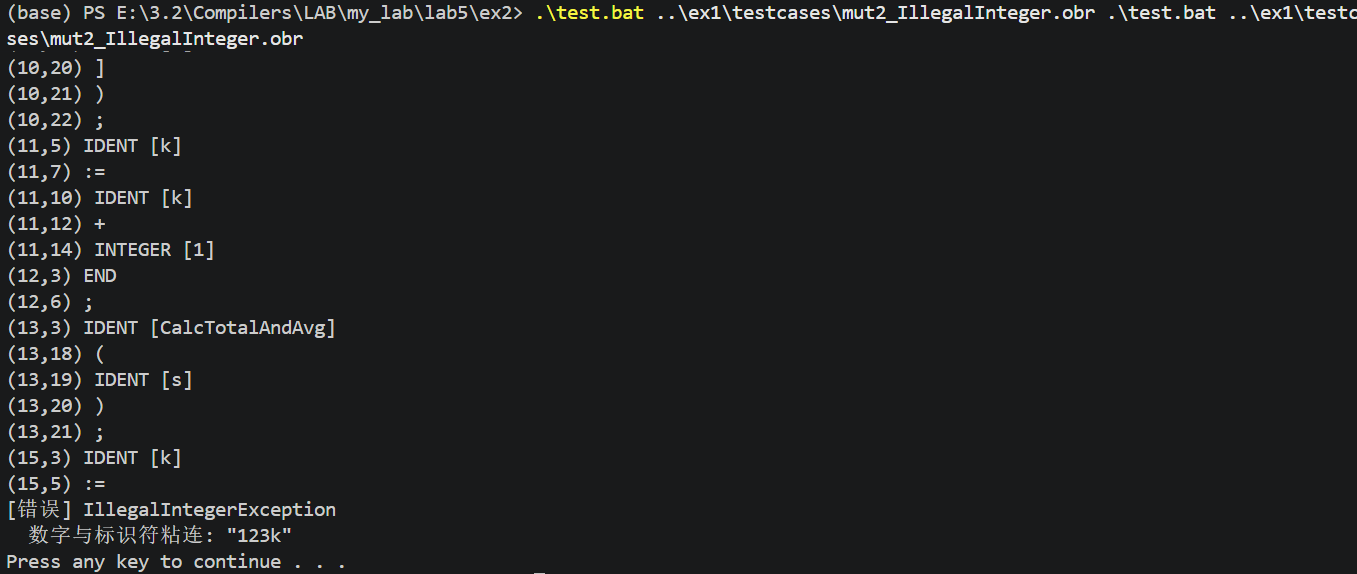
\includegraphics[width=0.9\textwidth]{img/2.png}
\caption{变异 2: IllegalInteger —— 数字标识符粘连 123k 被正确捕获}
\label{fig:mut2}
\end{figure}

\begin{figure}[H]
\centering
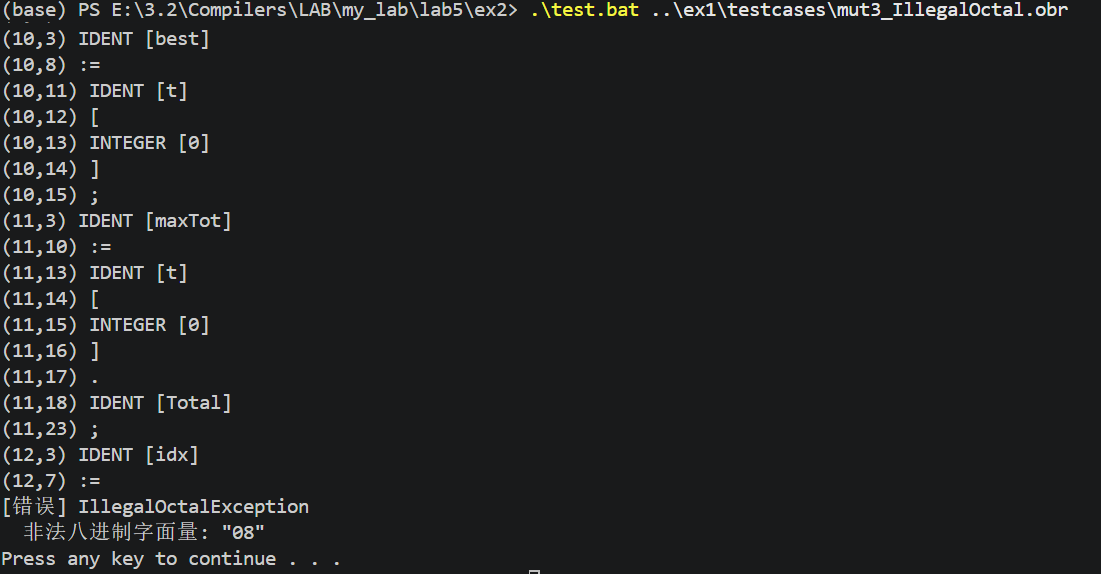
\includegraphics[width=0.9\textwidth]{img/3.png}
\caption{变异 3: IllegalOctal —— 非法八进制 08 被正确捕获}
\label{fig:mut3}
\end{figure}

\begin{figure}[H]
\centering
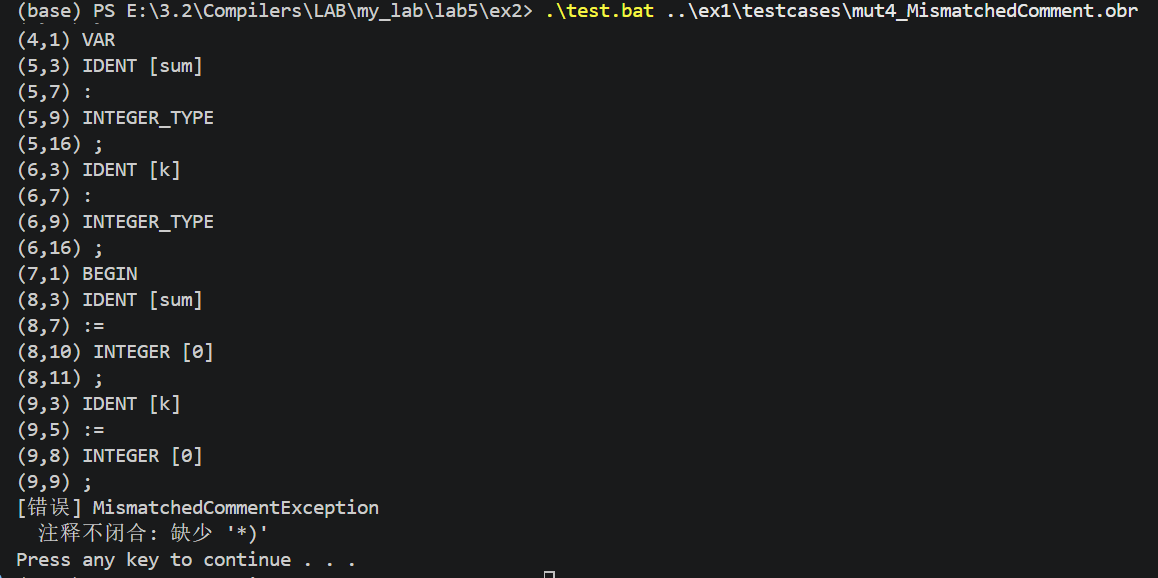
\includegraphics[width=0.9\textwidth]{img/4.png}
\caption{变异 4: MismatchedComment —— 注释不闭合被正确捕获}
\label{fig:mut4}
\end{figure}

\begin{figure}[H]
\centering
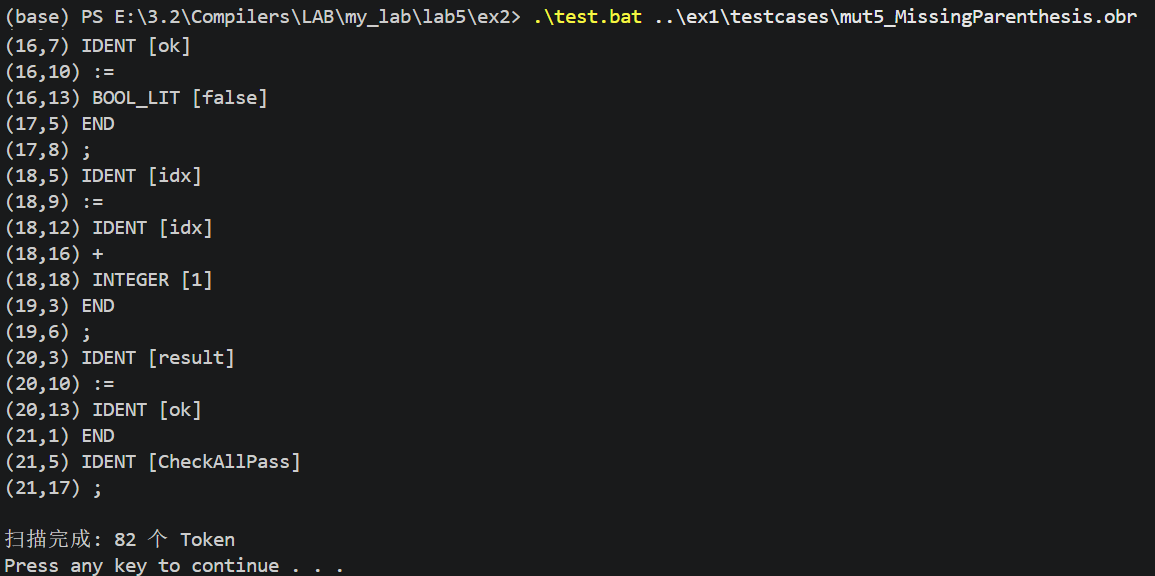
\includegraphics[width=0.9\textwidth]{img/5.png}
\caption{变异 5: MissingParenthesis —— 语法错误，词法阶段正常通过}
\label{fig:mut5}
\end{figure}

\begin{figure}[H]
\centering
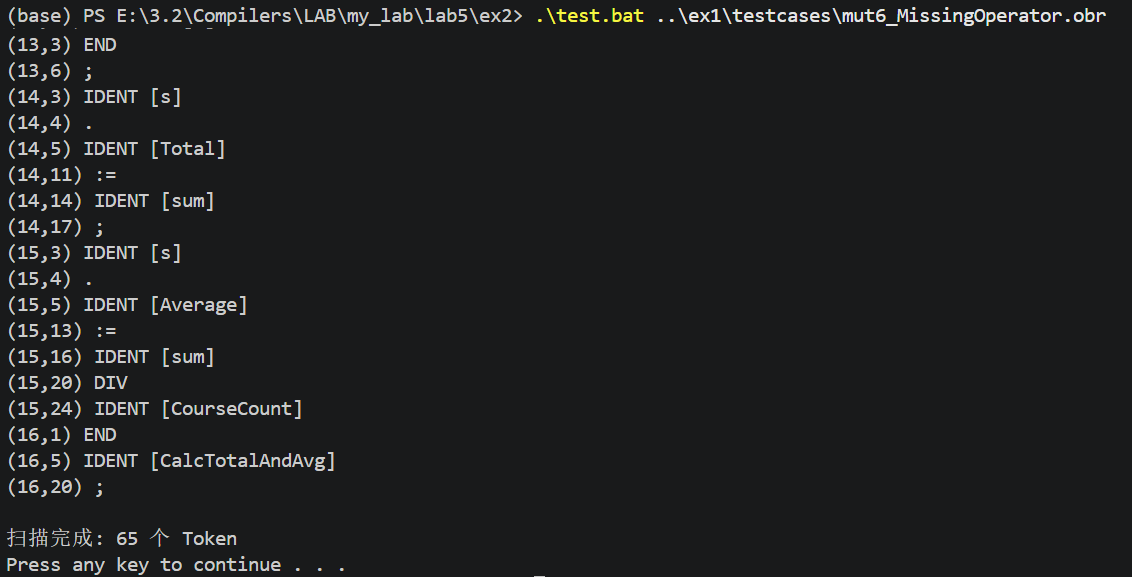
\includegraphics[width=0.9\textwidth]{img/6.png}
\caption{变异 6: MissingOperator —— 语法错误，词法阶段正常通过}
\label{fig:mut6}
\end{figure}

\begin{figure}[H]
\centering
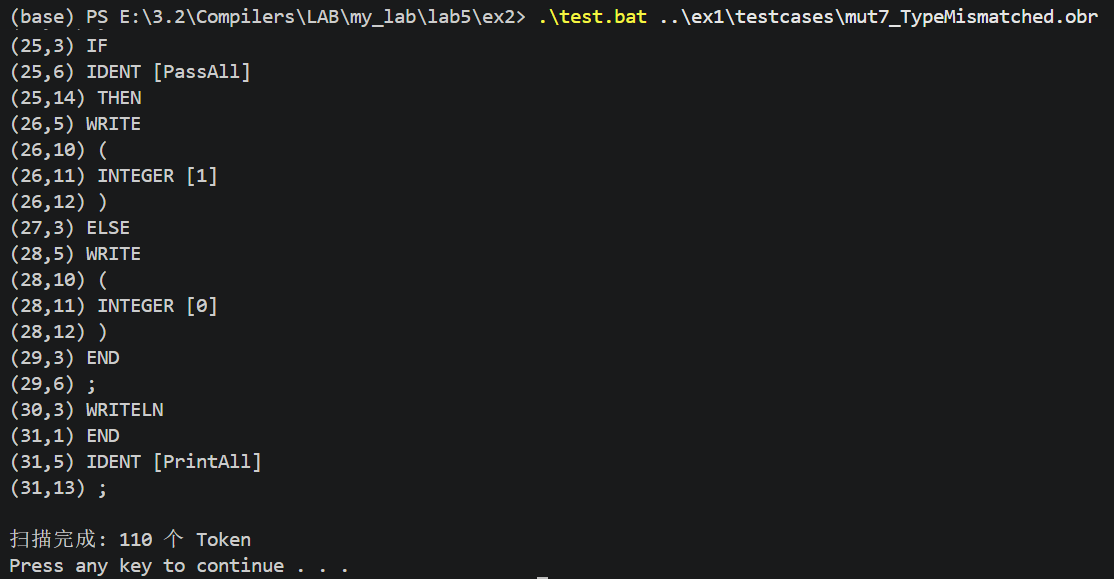
\includegraphics[width=0.9\textwidth]{img/7.png}
\caption{变异 7: TypeMismatched —— 语义错误，词法阶段正常通过}
\label{fig:mut7}
\end{figure}

\begin{figure}[H]
\centering
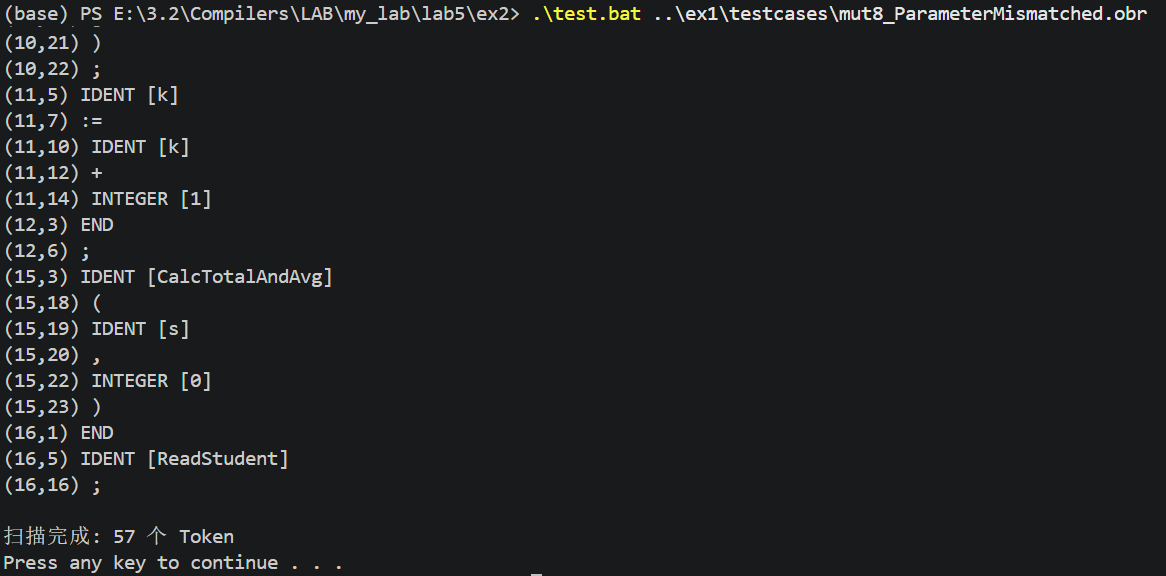
\includegraphics[width=0.9\textwidth]{img/8.png}
\caption{变异 8: ParameterMismatched —— 语义错误，词法阶段正常通过}
\label{fig:mut8}
\end{figure}

如上所示，变异 1--4 在词法分析阶段即被 OberonScanner 准确拦截并抛出对应异常，验证了
词法分析器对 IllegalSymbol、IllegalInteger、IllegalOctal、MismatchedComment 四类错误
的检测能力。变异 5--8（语法/语义层错误）在词法阶段正常通过，留待语法分析器和语义分析
器进一步处理，体现了编译器前端分层过滤的工程架构。

\subsection{Javadoc 设计文档生成}

本实验额外提供了 \texttt{gendoc.bat} 脚本，调用 JDK 自带的 \texttt{javadoc} 工具
对 \texttt{src/} 下所有手写 Java 源码（Token.java、OberonScannerTest.java 及 5 个
自定义异常类）生成 HTML 格式的 API 设计文档，输出至 \texttt{doc/} 目录。自动生成
的文档以标准 Javadoc 样式呈现类层次结构、字段说明和方法签名，便于后续维护与查阅。

\section{实验心得与体会}

JFlex 的宏系统（Macros）大幅提升了规则的模块化程度——先定义 \texttt{Letter}、
\texttt{Digit}、\texttt{Identifier} 等基础宏，再在规则段以组合形式引用，使得整体规则
清晰可读。而在遇到"标识符长度 24"和"八进制非法数字"这类无法用纯正则表达的约束时，
词法动作中的 Java 代码注入展现了声明式框架与命令式编程协作的能力。

自定义异常体系（\texttt{IllegalSymbolException}、\texttt{IllegalIntegerException}、
\texttt{IllegalOctalException}、\texttt{MismatchedCommentException}、
\texttt{IllegalIdentifierLengthException}）的设计使我意识到：词法分析器不仅是
"将字符流切分为 Token 流"的机械过程，更是一个\textbf{具有语义判断能力的前端过滤器}。
通过在词法阶段即精确报告错误的行列号与具体原因，可以为后续语法分析和用户错误定位提供
精准的上下文信息。

此外，对 JFlex/JLex/Flex 三种工具的对比分析让我理解了一个深刻的原则：\textbf{工具的选择
决定了编译器的上限，但规则的设计决定了编译器的下限}。JFlex 凭借优化后的 DFA 压缩算法和
完整的 Unicode 支持提供了性能与灵活性的保障，但若规则定义不当（如漏掉注释状态中对 EOF
的处理），仍会在边界 case 中产生漏检。
\end{document}
